% ------------------------------------------------------------------
\documentclass[12 pt]{article} % A4 paper set by geometry package below
\pagenumbering{arabic}
\setlength{\parindent}{10 mm}
\setlength{\parskip}{12 pt}

% Nimbus Sans font should be reasonably legible
\usepackage{helvet}
\renewcommand{\familydefault}{\sfdefault}
\usepackage[T1]{fontenc}  % Without this \textsterling produces $

% Section header spacing
\usepackage{titlesec}
\titlespacing\section{0pt}{12pt plus 4pt minus 2pt}{0pt plus 2pt minus 2pt}
\titlespacing\subsection{0pt}{12pt plus 4pt minus 2pt}{0pt plus 2pt minus 2pt}
\titlespacing\subsubsection{0pt}{12pt plus 4pt minus 2pt}{0pt plus 2pt minus 2pt}

\usepackage{amsmath}
\usepackage{amssymb}
\usepackage{graphicx}
\usepackage{verbatim}    % For comment
\usepackage[paper=a4paper, marginparwidth=0 cm, marginparsep=0 cm, top=2.5 cm, bottom=2.5 cm, left=3 cm, right=3 cm, includemp]{geometry}
\usepackage[pdftex, pdfstartview={FitH}, pdfnewwindow=true, colorlinks=true, citecolor=blue, filecolor=blue, linkcolor=blue, urlcolor=blue, pdfpagemode=UseNone]{hyperref}

% Put module code and last-modified date in footer
\usepackage{fancyhdr}
\pagestyle{fancy}
\fancyhf{}
\renewcommand{\headrulewidth}{0pt}
\cfoot{{\small \thisunit}\hfill \thepage\hfill {\small \moddate}}

% Hopefully address Canvas complaints about pdf tagging
%\usepackage[tagged]{accessibility}
\hypersetup {
  pdfauthor={David Schaich},
  pdftitle={Statistical Physics Tutorial Problem},
}
% ------------------------------------------------------------------



% ------------------------------------------------------------------
% Shortcuts
\newcommand{\la}{\ensuremath{\lambda} }
\newcommand{\lath}{\ensuremath{\la_{\mathrm{th}}} }
\newcommand{\Om}{\ensuremath{\Omega} }
% ------------------------------------------------------------------



% ------------------------------------------------------------------
\begin{document}
\newcommand{\thisunit}{MATH327 Tutorial (Mixing)}
\newcommand{\moddate}{Last modified 4 Mar.~2022}
\begin{center}
  {\Large \textbf{MATH327: Statistical Physics, Spring 2022}} \\[12 pt]
  {\Large \textbf{Tutorial problem \ --- \ Mixing entropy}} \\[24 pt]
\end{center}

Let's consider a slight variation to the particle exchange thought experiment we worked through in class.
We again begin with two canonical ideal gases, initially separated by a wall, each with $N$ particles in volume $V$ at temperature $T$.
\textbf{All} $2N$ particles have identical physical properties, \textit{except} that those initially in the left compartment (the ``reds'') are distinguishable from those in right compartment (the ``blues'') by their colour.
Call this initial system $\Om_0$.
We have already computed its entropy $S_0 = 2S_I(N, V) = 5N + 2N\log\left(\frac{V}{N\lath^3}\right)$, where $\lath = \sqrt{2\pi\hbar^2 / (mT)}$.

We then carry out the procedure of removing the wall, allowing the combined system to reach thermodynamic equilibrium, and then re-inserting the wall to re-separate the two systems.
Call the combined system $\Om_C$ with entropy $S_C$.
As discussed in class, it's safe to assume that $N$ particles end up in each of the two re-separated systems.
However, red and blue particles can now appear in either of the two re-separated systems.
Call this final system $\Om_F$ with entropy $S_F$.
The initial and final systems are illustrated by the figure below.

\begin{center}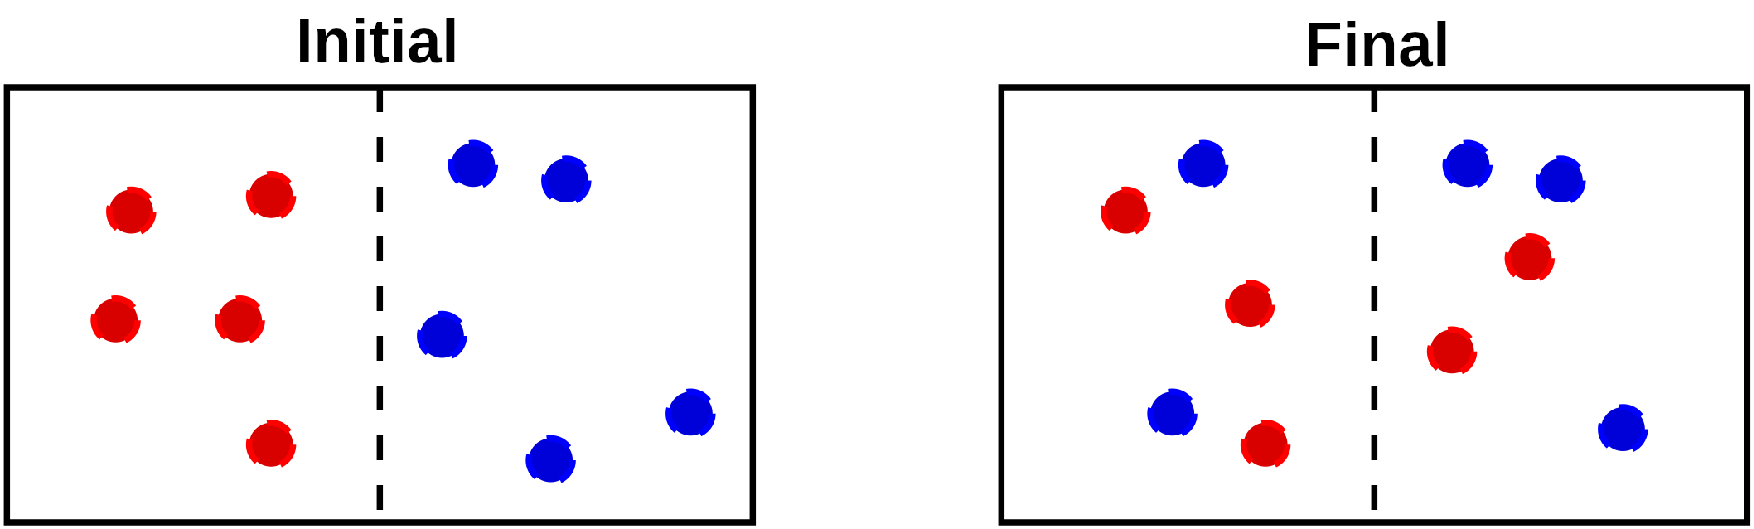
\includegraphics[width=0.8\textwidth]{figs/mix.pdf}\end{center}

The first task is to compute the mixing entropy $S_{\text{mix}} = S_C - S_0$, where in the combined system $\Om_C$ we now have two sets of $N$ indistinguishable particles, but can distinguish between the two sets.
The starting point is the partition function
\begin{equation*}
  Z_C = \frac{1}{N!} \frac{1}{N!} Z_1^{2N} = \frac{1}{N!} \frac{1}{N!} \left(\frac{2V}{\lath^3}\right)^{2N},
\end{equation*}
where $Z_1 = 2V / \lath^3$ is the single-particle partition function.

The second task is to compute the final entropy $S_F$, to see whether $S_F \geq S_C$ as demanded by the second law of thermodynamics.
We can break this up into two steps.
The first of these is to compute the partition function $Z_F$ of the two re-separated systems (each with $N$ particles), summing over all ways of dividing the red and blue particles between them.
The following special case of the \href{https://en.wikipedia.org/wiki/Zhu_Shijie}{Zhu}--\href{https://en.wikipedia.org/wiki/Alexandre-Theophile_Vandermonde}{Vandermonde} \href{https://en.wikipedia.org/wiki/Vandermonde's_identity}{identity} may be useful for this step:
\begin{equation*}
  \sum_{k = 0}^N \binom{N}{k}^2 = \binom{2N}{N}.
\end{equation*}

Finally, use your result for $Z_F$ to determine the final entropy $S_F$.

\end{document}
% ------------------------------------------------------------------
